\chapter{A razor search for dark matter at 100 TeV}\label{ch:DM_100_TeV}

In 1933, the Swiss astronomer Fritz Zwicky turned his telescope to the night sky to measure the velocities of galaxies in a particular galaxy cluster known as the Coma cluster. He discovered that the visible matter in this cluster could not account for the speeds at which the galaxies were moving. He postulated that there must be some matter that does not emit light, but has mass and interacts only gravitationally with known matter. He termed this `Dunkle materie', or \emph{dark matter}. The evidence for dark matter has only continued to grow since then, and we now know that there is far more of it in the universe than there is regular, or \emph{baryonic} matter. The nature of dark matter is one of the most compelling mysteries in physics today.

Over the years, there have been many dark matter candidates\footnote{For a while, it was debated whether the effects of dark matter could instead be explained by a deviation of the gravitational force from the usual inverse square law at large length scales. This theory was termed Modified Newtonian Dynamics, or MOND \citep{Milgrom1983}. However, it was shown in 2006 \citep{Clowe2006} that MOND was fundamentally incompatible with the data from the bullet cluster.}, but the most widely accepted view today is that dark matter is comprised of a completely new kind of particle \footnote{Of course, this is not the only possibility. Instead of a single dark matter candidate particle, there could be a 'dark sector' comprised of multiple particles and interactions between them. See (DDM papers) for developments along this line.} that interacts only weakly with the particles of the Standard Model and moves at at non-relativistic speeds.

\strictpagecheck
\begin{figure}
  \begin{sidecaption}
    {Rotation curves for a number of spiral galaxies. \citep{Sofue2001}}
  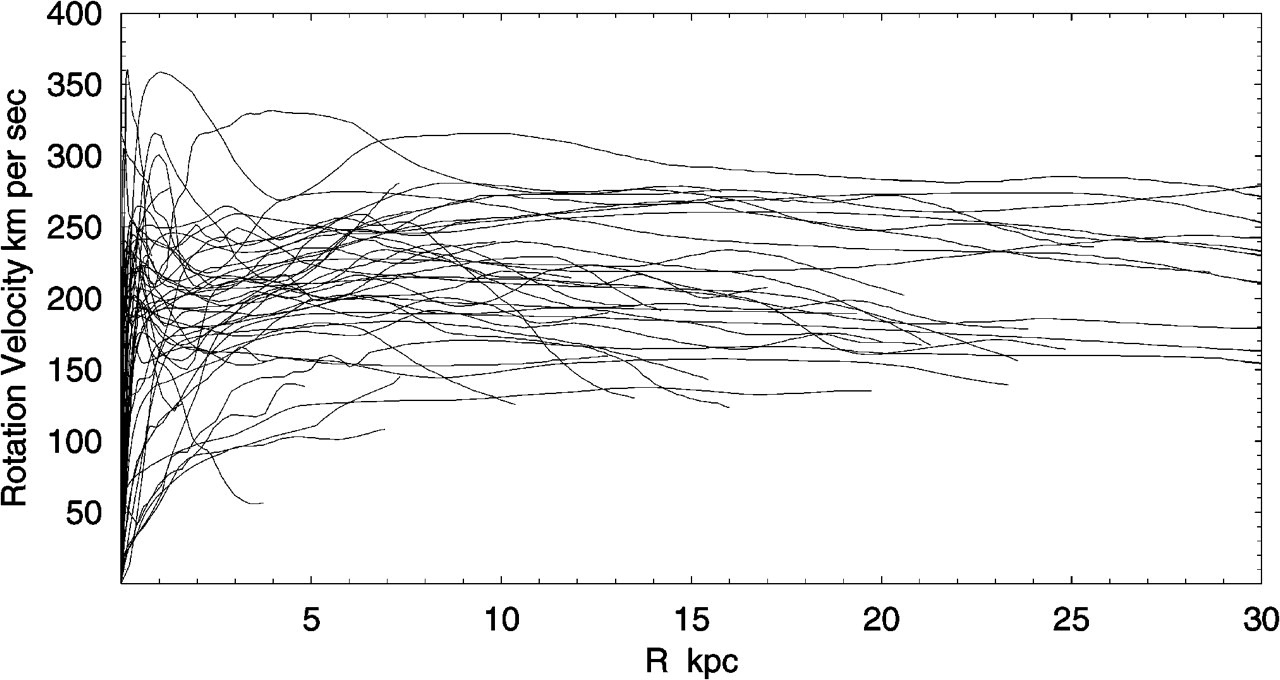
\includegraphics[width=\textwidth]{images/rotation_curves}
\end{sidecaption}
\end{figure}
One of the most tantalizing clues to the nature of dark matter is the so-called 'WIMP miracle' - the remarkable coincidence that the observed dark matter density in the universe can arises naturally from a particle with mass and couplings comparable to the weak scale. This raises the hope that such particles might feasibly be detected at colliders or direct detection experiments.
\section{Dark matter, three ways}\label{dark-matter-three-ways}
\begin{marginfigure}
  \centering
  \begin{tikzpicture}
    \begin{feynman}
      \vertex (v1) {\(\chi\)};
      \vertex [right=of v1] (v2){\(SM\)};
      \vertex [below=of v1] (v3){\(\chi\)};
      \vertex [right=of v3] (v4){\(SM\)};
      % Placing vertex v between v1 and v4
      \vertex [blob] (v) at ($(v1)!0.5!(v4)$) {};
      \vertex [above=of v] (l2){Indirect};
      \vertex [below=of v] (l3){Collider};
      \diagram*{
        (v1) -- (v),
        (v2) -- (v),
        (v3) -- (v),
        (v4) -- (v),
      };
      \draw [->] ($(v1.west) + (-2mm,0)$) -- ($(v3.west) + (-2mm,0)$) node [sloped,midway,above,rotate=180] {Direct};
      \draw [->] ($(v1.north) + (0,2mm)$) -- ($(v2.north) + (0,2mm)$);
      \draw [->] ($(v4.south) + (0,-2mm)$) -- ($(v3.south) + (0,-2mm)$);
    \end{feynman}
  \end{tikzpicture}
  \caption{DM detection, three ways}
  \label{fig:dm_annihilation}
\end{marginfigure}

There are three main methods of detecting WIMP dark matter. The first, direct detection, involves constructing a well shielded, giant vat of a relatively inert substance, and waiting for dark matter particles to interact with that substance. The second, termed indirect detection, involves searching for signs of dark matter particles annihilating each other in the cosmos. The third method, collider detection, involves producing dark matter through high energy particle collisions and searching for their associated signatures. The first two methods place relatively stringent constraints on the nature of dark matter, but have their own limitations. The smallest interaction cross-section between dark matter and regular matter that direct detection can measure is limited from below by the background of neutrinos from the sun, though there are creative methods that are being developed to deal with this background. Indirect detection suffers from large astrophysical uncertainties. Collider detection, therefore, is competitive with, and can even possibly surpass the other two methods.

\newcommand{\cb}{ c_\beta}
\newcommand{\cw}{ c_W}
\newcommand{\sinb}{ s_\beta}
\newcommand{\sw}{ s_W}
\newcommand{\mz}{ m_Z}

%The non-SM interactions in our signal process are the higgsino-bino-$Z$ and the higgsino-bino-$h$ interactions. To determine their coupling, we can inspect the structure of the MSSM. We will first examine the gauge interactions of higgsino and bino gauge eigenstates. Upon doing this, it will be apparent that there are no interaction terms containing both pure higgsinos and pure binos. The reason is that electroweak symmetry breaking induces mixing among the neutralinos. After this, we will move on to the coupling involving the SM Higgs boson, and see how it is obtained. 
%Inserting the covariant derivatives into the kinetic terms will yield the interaction terms. Each of the fields $H_u$ and $H_d$ can be interpreted as the scalar field $\phi$ in \eqref{eq:phi1} and \eqref{eq:phi2}. Similarly, the supersymmetrizations of $H_u$ and $H_d$,
%\[\widetilde{H_u} = \begin{pmatrix}\widetilde{H_u}^+\\\widetilde{H_u}^0\end{pmatrix};
%\widetilde{H_d} = \begin{pmatrix}\widetilde{H_d}^0\\\widetilde{H_d}^-\end{pmatrix}\]
%can be equated with the field $\psi$ in \eqref{eq:psi}. The component fields of these are called \emph{higgsinos}. Once we insert the generators and associated gauge fields for the $SU(2)_L\times U(1)_Y$ symmetry in the covariant derivatives, and mix the gauge fields in the manner dictated by electroweak symmetry breaking, the gauge interactions of the higgs and higgsino fields look a lot like the SM interactions. In fact, they will have the same strength. Since we are interested in neutral higgsino-like NLSPs for our signal process, let us isolate their particular interaction terms:
%\[\frac{g}{\cos\theta_W}Z_\mu\left(\widetilde{H_u}^{0\dagger}\overline{\sigma}^\mu \widetilde{H_u}+
%\widetilde{H_d}^{0\dagger}\overline{\sigma}^\mu \widetilde{H_d}\right)\]
%Now let us turn to the interactions of gauge supermultiplets. A generic gauge supermultiplet will consist of a gauge boson $A_\mu^a$ and its two-component Weyl fermion superpartner, the \emph{gaugino} $\lambda^a$. The SM gauge bosons reside in such gauge supermultiplets, and so the index $a$ runs over the adjoint representation of the relevant gauge group. The gauge interactions of gauginos can be extracted from their kinetic term in the Lagrangian:
%\[\mathcal{L}_{\text{gaugino,kinetic}} = i\lambda^{a\dagger}\overline{\sigma}^\mu\nabla_\mu\lambda^a\]
%where the covariant derivative is given by
%\[\nabla_\mu\lambda^a = \partial_\mu\lambda^a + gf^{abc}A_\mu^b\lambda^c.\]
%The factors $f^{abc}$ represent the structure constants of the gauge group. Thus, the interaction term would look like:
%\[ig\lambda^{a\dagger}\overline{\sigma}^\mu f^{abc}A_\mu^b\lambda^c\]
%The bino $(\widetilde{B}^0)$ is the superpartner of the SM gauge boson associated with the $U(1)_Y$ (hypercharge) gauge symmetry. Thus, it will transform in the adjoint representation of $U(1)_Y$ as well. However, this implies that there can never be a interaction vertex containing a bino and a gauge boson, since the structure constants for $U(1)_Y$ are all simply 0. In addition, we have previously seen that examining the chiral supermultiplet conaining the higgsino does not yield a neutral higgsino-bino-$Z$ vertex either. The reason that we can consider such a vertex in our signal process is due to the fact that electroweak symmetry breaking induces mixing among neutral higgsinos, binos, and the neutral wino $(\widetilde{W}^0)$, the superpartner of the $W_\mu^3$ gauge field associated with the SM $SU(2)_L$ gauge symmetry that mixes with $B_\mu$ to form the $Z$ boson and photon.

% Motivation: dark matter is interesting
The existence of dark matter is unambiguous evidence of the need for new physics beyond the Standard Model (SM) of particle physics. Indeed, given that there is far more dark matter in the universe than there is baryonic matter, determining its precise nature is one of the most exciting challenges in physics today. It is widely believed that dark matter is comprised of stable weakly interacting massive particles. These particles arise naturally in many extensions of the SM. Of these extensions, one of the most studied is the Minimal Supersymmetric Standard Model (MSSM). For a detailed review, see \citep{Martin1997}. In the MSSM, the lightest supersymmetric partner (LSP) is predicted to be absolutely stable, making it a good candidate for dark matter. The identity of the LSP is determined by the mass hierarchy of the superpartners, which in turn depends on how supersymmetry is broken. However, taking into account experimental constraints and phenomenological considerations, the lightest neutralino emerges as the most attractive candidate for the LSP \citep{Bertone2005a}. 

% Why go beyond the MSSM?
Despite the attractive simplicity of natural SUSY, it is under siege from recent  data from the Large Hadron Collider (LHC). A compelling alternative scenario comes in the form of split supersymmetry  \citep{Wells:2003tf, Dimopoulos2004, Giudice2005}. In this scenario, the lightest superpartners are the fermionic ones (gauginos and higgsinos), on the scale of 1-10 TeV, while the scalar superpartners can be much heavier, on the scale of 100 - 1000 TeV. In exchange for accepting some level of fine-tuning, we obtain numerous benefits, including the suppression of flavor-changing neutral currents and greater compatibility with data from CP-violation experiments.

% Why a 100 TeV collider?
The most interesting regions of the split SUSY parameter space lies beyond the reach of the LHC. Consider, for example the case in which the dark matter candidate is a nearly-pure bino. Even though the simplicity of its gauge singlet structure makes it an attractive DM candidate, It is well known that heavy bino LSPs heavier than about 200 GeV result in an overabundance of dark matter in the universe, in conflict with experimental observations. However, if the bino is nearly mass-degenerate with another supersymmetric particle, such as the gluino, stau, or a squark, it can coannihilate with it, thereby reducing the dark matter abundance to acceptable levels. Coannihilation with a gluino would raise the acceptable bino mass to $\sim 7$ TeV, and coannihilation with a stop or squark raises the acceptable bino mass to $\sim 2$ TeV. Bringing one of these particles down to the low-energy spectrum should not affect the branching ratio of the higgsinos too much. Gluino coannhilators would not change the branching ratios of the neutral higgsinos, since they are uncharged under $SU(3)_c$\footnote{But doing so would reduce the importance of electroweak search channels in comparison, as gluinos would then be abundantly produced.}. Higgsino-fermion-sfermion couplings are Yukawa-like, and are proportional to the mass of the fermion in the interaction vertex. Thus, this coupling will be relatively small (with the possible exception of the higgsino-top-stop case). In this paper, we will simply assume that a scalar can be brought down into the low-energy spectrum to be nearly mass-degenerate with the bino, thus satisfying the relic density requirement. Such heavy binos are out of the reach of the 14 TeV LHC, but well within the reach of a 100 TeV collder. 
\begin{marginfigure}
  \feynmandiagram [layered layout, vertical = a to b]{
  bino [label = \(\tilde{B}^0\)] -- [fermion] a -- [anti fermion] tau [label = \(\tau\)],
  stau [label = \(\widetilde{\tau}\)] -- [anti charged scalar] b -- [boson] Z [label = \(Z\)],
  {[same layer] a -- [charged scalar, edge label=\(\widetilde{\tau}\)] b},
};
\end{marginfigure}
%For example, if dark matter consists of nearly pure winos\footnote{Throughout this paper, we will refer to wino-like, higgsino-like, or bino-like neutralinos as simply winos, higgsinos, and binos.} or higgsinos, \Shufang{Higgsino} \Adarsh{What did you want me to change here?}  they would have to be extremely heavy (3.1 TeV and 1 TeV respectively) to be consistent with the observed relic density of dark matter in the universe. However, the LHC, with its center of mass energy of 14 TeV, is expected to discover winos only up to a mass of about 500 GeV, and higgsinos up to a mass of about 200 GeV.  \Shufang{reference here.} \Adarsh{These limits are from [6].}  In contrast, a 100 TeV proton-proton collider would be able to probe directly produced thermal winos \citep{Low2014}, as well as thermal higgsinos produced in cascade decays \citep{Gori:2014oua}.

Apart from being able to probe thermal neutralino dark matter candidates, a 100 TeV collider would open up an immense number of physics opportunities not afforded to a 14 TeV collider \citep{Arkani-Hamed2015}. 
% Status of 100 TeV planning
Such a collider would be a natural next step after the LHC, and is being actively discussed in the particle physics community, with two major proposals being the FCC-hh by CERN \citep{FCC-hh}, and the SppC by IHEP in China \citep{CEPC}. Executing a project of this size requires an immense amount of planning, over many years. Now is an opportune time to begin to fully explore the physics potential of a 100 TeV collider. There have been a number of studies conducted already, and more are coming out in the literature on a regular basis. 
% Point to review papers for enumeration of studies
We will not attempt to enumerate them all, and instead point the interested reader to the references sections of the review papers \citep{Arkani-Hamed2015,Contino:2016spe,Golling:2016gvc,Mangano:2016jyj}.

This paper aims to add to the corpus an assessment of the prospects of finding pair-produced neutral higgsinos that decay to binos via intermediate $Z$ and $h$ bosons. Razor variables \citep{Rogan2010} were originally designed for searches involving two heavy, mass-degenerate pair-produced particles, each of which decays into a visible and invisible set of particles. This topology matches that of our search channel, making this set of variables a natural choice for our analysis.

Finding higgsinos has traditionally been more challenging than finding winos, due to their lower production rate - it is thus important to devise innovative strategies to do so. In addition, the higgsino mass parameter $\mu$ that governs the mass of the higgsino plays an important role in electroweak symmetry breaking \citep{Acharya2014}. This combination of NLSP (next-to-lightest supersymmetric partner) and LSP has been studied earlier in \citep{Gori:2014oua} with intermediate vector dibosons and multi-lepton final states. In this paper, however, we attempt to exploit the relatively high branching ratio of the SM Higgs boson to $b$ quarks, and choose the decay modes $Z\rightarrow ll$ and $h\rightarrow bb$ for the intermediate $Z$ and $h$ bosons in our search channel.  

At a 100 TeV collider, the backgrounds are going to be even larger than at the LHC. We will need to harness all the possible tools we can to deal with them. An ancillary goal of this paper is to investigate the potential for machine learning (ML) techniques to augment our analysis. with the advent of more powerful computers and simultaneous advances in the field of statistical learning in recent years, the usage of ML is rising in experimental particle physics. In fact, the discovery of the SM Higgs boson in 2012 was done with the help of neural networks \citep{ATLASCollaboration2012} and boosted decision trees \citep{CMSCollaboration2012}.

The rest of the paper is structured as follows. In section \ref{sec:model}, we describe our model and search channel in more detail, and list the existing experimental constraints on it. In section \ref{sec:analysis}, we describe our analysis strategies and results obtained for both the traditional cut-and-count analysis and the analysis performed with boosted decision trees. Finally, we conclude with the implications in section \ref{sec:conclusion}.

\section{Model and experimental constraints}\label{sec:model}

In this section, we will elaborate a little more on the structure of the neutralino sector in the MSSM (and by extension, split SUSY), motivate our chosen search channel, and review some of the relevant experimental literature and limits.

\subsection{The neutralino sector}
The neutralino sector consists of four mass eigenstates ($\tilde{\chi}_1^0,\tilde{\chi}_2^0,\tilde{\chi}_3^0,\tilde{\chi}_4^0$)  that are mixtures of the gauge eigenstates ($\tilde{B}^0,\tilde{W}^0,\tilde{H}_u^0,\tilde{H}^0_d$) - the bino, the wino, and the two neutral higgsinos. In the basis of these gauge eigenstates, the mass matrix of the neutralino can be written as

\[\mathbf{M}_{\tilde{N}}=
\begin{pmatrix}
  M_1 & 0 & -\cb\sw\mz & \sinb\sw\mz \\
  0 & M_2 & \cb\cw\mz & \sinb\cw\mz \\
  -\cb\sw\mz & \cb\cw\mz & 0 & -\mu \\
  \sinb\sw\mz & -\sinb\cw\mz & -\mu & 0
\end{pmatrix},\]

\noindent where $\sinb = \sin\beta, \cb = \cos\beta, \sw = \sin\theta_{W}$,  and  $\cw = \cos\theta_W$. The angle $\beta$ is a central parameter of the theory - it parameterizes the mixing between the two Higgs doublets, $\tilde{H}_u$ and $\tilde{H}_d$. It is defined as $\tan\beta = v_u/v_d$, where $v_u$ and $v_d$ are the vacuum expectation values of $H_u^0$ and $H_d^0$. The parameters $M_1$, $M_2$, and $\mu$ are the coefficients of bino, wino, and higgsino mass terms in the soft supersymmetry breaking Lagrangian.
This matrix can be diagonalized with the unitary matrix $\mathbf{N}$ to obtain 
\[\mathbf{N^*M_{\tilde{N}}N^{-1}} =
\begin{pmatrix}
  m_{\tilde{\chi}_1} & 0 & 0 & 0\\
  0 & m_{\tilde{\chi}_2} & 0 & 0 \\
  0 & 0 & m_{\tilde{\chi}_3} & 0 \\
  0 & 0 & 0 &  m_{\tilde{\chi}_4} \\
\end{pmatrix},
\]
where $m_{\tilde{\chi_i}}$ are the masses of the neutralino mass eigenstates. 

In the limit of $\mz \ll |\mu\pm M_1|, |\mu\pm M_2|,$ the mass eigenstates are, to good approximation, a nearly pure bino, $\tilde{B}^0$, with mass $M_1$, a nearly pure wino, $\tilde{W}^0$, with mass $M_2$, and nearly pure higgsinos $\tilde{H}^0_{1,2} = (\tilde{H}_u^0 \pm \tilde{H}_d^0)/\sqrt{2}$, with mass $|\mu|$\footnote{This limit is well-motivated, since we are considering heavy electroweakinos that are out of the reach of the LHC - the minimum mass of the higgsinos considered is 500 GeV, and the wino is decoupled to 3 TeV.}. 

The optimal search strategy for finding electroweakinos is highly dependent on the mass difference between them. Phenomenological collider studies on finding electroweakinos separated by about 0.1 - 50 GeV at a 100 TeV collider can be found in \citep{Low2014, Plehn2015, Berlin2015, Cirelli2014}, while well-separated spectra have been studied in \citep{Gori:2014oua, Acharya2014}.
So far, the well-separated spectra have been studied using multi-lepton channels, of the form 
\[pp\rightarrow \tilde{\chi}_\text{NLSP}\tilde{\chi}_\text{NLSP}\rightarrow VV + \tilde{\chi}_\text{LSP}\tilde{\chi}_\text{LSP}\rightarrow 2l/3l + \slashed{E}_T +  \tilde{\chi}_\text{LSP}\tilde{\chi}_\text{LSP}\]
where $\tilde{\chi}_\text{NLSP}$ can be a neutralino or chargino, and $\tilde{\chi}_\text{LSP}$ is the lightest neutralino. These searches work well since the large mass difference between the electroweakinos can lead to energetic leptons that can be easily identified. Among the multi-lepton searches, the trilepton searches (with $W$ and $Z$ as the intermediate dibosons) have the best reach, due to the high production cross-section of chargino-neutralino pairs combined with the large reduction in $t\overline{t}$ and QCD backgrounds obtained by requiring three leptons. Multilepton searches with $Zh$ and $ZZ$ as the intermediate dibosons are unlikely to be as powerful, due to the lower pair-production cross-section of neutral higgsinos, combined with the low branching ratio of $Z$ to leptons. However, if we move beyond multilepton searches, the channel with $Zh$ as the intermediate dibosons emerges as a possible competitor to the $WZ$ channel. If the $Z$ decays leptonically and $h$ decays to a pair of $b$s, then after applying the relevant branching ratios, the signal cross sections become comparable (for details, see table \ref{tab:xsections}). 
In this paper, we will focus on a well-separated electroweakino spectrum, with $M_2 \gg |\mu|,M_1$, and study the process:
\[pp\rightarrow \tilde{\chi}_{2}^{0}\tilde{\chi}_{3}^{0}\rightarrow (Z\tilde{\chi}_1^{0})(h\tilde{\chi}_1^{0})\rightarrow ((l^+l^-)\tilde{B}^{0})((b\overline{b})\tilde{B}^0),\]
which is manifested at colliders as a final state with two \emph{b}-jets, two same flavor, opposite sign leptons, and missing transverse energy. The main backgrounds for this process are: $t\overline{t}$, $tbW$ with the $b$ and $W$ not coming from a $t$, and $bbWW$ with no intermediate $s$-channel top quarks. See \autoref{fig:feynman_diagrams} for representative Feynman diagrams for the signal and background processes. The typical pair-production cross section for the higgsino-like NLSPs is on the order of less than 10 fb for $|\mu|>1$ TeV, as can be seen in figure \ref{fig:xsection_plot}.  

\begin{table}
\centering
\begin{tabular}{l|rr}
\toprule
Stage & $\tilde{\chi}_{2,3}^0\tilde{\chi}^\pm_{2}$ & $\tilde{\chi}^0_{2}\tilde{\chi}^0_{3}$\\
\midrule
Pair production cross section & 60 fb & 16 fb\\
Intermediate diboson contribution & ($WZ$) 30 fb  & ($Zh$) 8 fb \\
Applying $BR(W\rightarrow l\nu)$, $BR(Z\rightarrow ll)$ \& $BR(h\rightarrow bb)$ & 0.42 fb & 0.32 fb\\
\bottomrule
\end{tabular}
\caption{Comparison of cross-sections for $(\tilde{\chi}_{2,3}^0\tilde{\chi}^\pm_{2})$ and $(\tilde{\chi}^0_{2}\tilde{\chi}^0_{3})$, for $|\mu|\approx 1$ TeV, at a 100 TeV $pp$ collider. The pair-production cross sections are taken from \citep{Gori:2014oua}, and the branching ratios are taken to be the same as the SM ones listed in the PDG \citep{Olive2016}.}
\label{tab:xsections}
\end{table}

\begin{figure}[h]
\centering
\includegraphics{images/xsection_plot.pdf}
\caption{Higgsino pair production cross section, for a bino mass of 25 GeV.}
\label{fig:xsection_plot}
\end{figure}

\begin{figure}%
\centering
\parbox{.21\textwidth}{%
    \includegraphics[width=0.21\textwidth]{images/signal.pdf}%
}
\parbox{.21\textwidth}{%
    \includegraphics[width=0.21\textwidth]{images/tt.pdf}%
}
\parbox{.27\textwidth}{%
    \includegraphics[width=0.27\textwidth]{images/tbW.pdf}%
}
\parbox{.27\textwidth}{%
    \includegraphics[width=0.27\textwidth]{images/bbWW.pdf}%
}
\label{fig:feynman_diagrams}
\caption{From left to right, the representative Feynman diagrams of the signal process, the dominant $tt$ background, $tbW$ without a top quark in the
$s$-channel, and $bbWW$ without a top quark in the $s$-channel. (Generated using \cite{Ellis2016}.)}%
\end{figure}

\subsection{Couplings and branching ratios}

The mixing of the neutralino gauge eigenstates gives rise to complicated expressions for the couplings involving the mass eigenstates. For consistency, We use SUSY-HIT to calculate the branching ratios $BR(\tilde{\chi}_{2,3}^0\rightarrow h\tilde{\chi}_1^0)$,$BR(\tilde{\chi}_{2,3}^0\rightarrow Z\tilde{\chi}_1^0)$, and $BR(h\rightarrow bb)$. For all our benchmark points, we decouple the neutral wino, setting $M_2 = 5$ TeV.

\subsection{Review of experimental searches and limits}

While the majority of the existing searches for supersymmetry focus on gluino pair production, there are a number of analyses involving electroweakino pair production as well, which we will attempt to briefly review here. 
Searches involving multiple leptons and missing energy $(2l/3l/4l +\slashed{E}_T)$ in the final state are described in \citep{ATLAS:2016uwq,ATLAS:2016soo,Khachatryan:2014qwa,Chatrchyan:2012pka}, assuming a wino-like NLSP and a bino-like LSP. The best reach is obtained in the $4l$ channel, with NLSP masses up to 1.14 TeV excluded for LSP masses greater than about 500 GeV. The trilepton channel is a close second-best, with NLSP masses up to 1 TeV excluded for a massless LSP. Both of these results have been calculated with 13.3 $fb^{-1}$ of 13 TeV LHC data by ATLAS. 

Topologies with one or two hadronically-decaying tau leptons and missing energy in the final state have been studied in \citep{ATLAS:2016ety,Khachatryan:2016trj}, with the greatest reach obtained by ATLAS in \citep{ATLAS:2016ety}, using 13 TeV data - they are able to exclude wino-like NLSPs up to a mass of 700 GeV for a massless bino-like LSP. 

Photon signatures $(\gamma\gamma/\gamma b/\gamma j/\gamma l/\gamma j j + \slashed{E}_T)$ been used to probe gauge mediated supersymmetry breaking  models in \citep{Chatrchyan:2012bba,CMS:2015loa,Aad:2015hea,Khachatryan:2015exa,Khachatryan:2016hns}. Winos are excluded below 710 GeV for nearly binos that are nearly mass-degenerate with them in \citep{Khachatryan:2016hns}. The study \cite{Aad:2015hea} excludes winos up to a mass of 590 GeV in the final state $\gamma\gamma + \slashed{E}_T$.  The final state $\gamma l + \slashed{E}_T$ is used to exclude winos up to 360 GeV in \citep{CMS:2015loa}. 

Searches with a combination of leptons and jets in the final states can be found in \citep{Aad:2014vma,Khachatryan:2015kxa,Khachatryan:2014mma}. Winos up to 465 GeV are excluded in the $2l + 0/2j$ final states in \citep{Aad:2014vma}. A compressed mass spectrum is studied in \citep{Khachatryan:2015kxa}, with a mass difference of about 50 GeV between winos and binos. This study uses the vector boson fusion channel, with a final state of $2l + 2j + \slashed{E}_T$, and excludes winos up to a mass of 170 GeV. Of particular interest to us is the analysis in \citep{Khachatryan:2014mma}, where higgsinos can be excluded up to a mass of 380 GeV using the $bbll + \slashed{E}_T$ final state, but cannot be discovered in any region of the relevant parameter space. As we shall see, a 100 TeV collider will enable us to greatly improve upon these limits.

\section{Analysis Details}\label{sec:analysis}

In this section, we will describe out strategies for both the traditional cut-and-count analysis, as well as the analysis carried out with boosted decision trees. 

\subsection{Simulation}\label{simulation}

We simulated parton-level events using \texttt{MadGraph5 v2.3.2.2} and \texttt{MadEvent} \citep{Alwall2014}, then passed those events to Pythia 6 \citep{Sjostrand2006} for showering and hadronization. Finally, we used \texttt{Delphes 3} \citep{DeFavereau2014a} to perform a fast, parametrized detector simulation, with the detector card devised by the FCC-hh working group\footnote{\url{https://github.com/HEP-FCC/FCCSW/tree/master/Sim/Sim/Delphes/Interface/data}}. For the backgrounds, we allowed up to one additional jet in the final state, to approximate NLO QCD effects, and performed MLM matching with the \texttt{xqcut} parameter set to 40 GeV. The Higgsino pair production cross sections were calculated using \texttt{Prospino2} \citep{Beenakker1999}. To decouple the wino, we set its mass parameter $M_2$ to 3 TeV.

One of the challenges we faced while performing this analysis was dealing with the sheer number of background events to generate and analyze. At a 100 TeV collider, the background cross-sections grow very large compared to their 14 TeV counterparts. For example, the cross section for the inclusive production of top quark pairs increases from $\sim975$ pb (N$^{3}$LO) to $\sim34,000$ pb (NLO) \citep{Mangano:2016jyj}, that is, increasing the collision energy by about seven times increases the number of events by a factor of more than 30! Multiplying this by 3 ab$^{-1}$ (the expected integrated luminosity from the first 10 years of running the FCC), gives us 96 billion top pair production events. Simulating this many events would require enormous amounts of computing time as well as huge amounts of storage. To alleviate the first problem, we generated events on the University of Arizona cluster, leveraging the power of many computing nodes to perform event generation simultaneously. But this alone would not be enough. 

Since we expect our signal process to have a dilepton resonance from an on-shell $Z$ boson, we restricted the phase space for event generation for backgrounds to the region where the invariant mass of dilepton pairs lies between 80 and 100 GeV. Additionally, the bino dark matter that escapes the detector would result in a large amount of missing transverse energy ($\slashed{E}_T$), so we required a minimum $\slashed{E}_T$ of 100 GeV at the parton level for the backgrounds as well. 

At the reconstructed level, we relaxed the lepton isolation criterion in the \texttt{Delphes} detector card from $\Delta R_{min}$ from 0.4 to 0.05. This is motivated by the fact that due to the large mass difference between the higgsino NLSP and the bino LSP in our search channel, the intermediate $Z$ bosons will be highly boosted, and the leptons to which they decay will be highly collimated. The value of 0.05 is consistent with what is suggested in previous 100 TeV studies (\citep{Acharya2014,Gori:2014oua,Bramante2015}) and will allow for easier comparison between strategies.


\subsection{Rectangular cuts}\label{event-selection}

For the cut-and-count analysis, we implemented successive one-dimensional cuts on the variables listed below, using the MadAnalysis 5 package \citep{Conte2013}.

\begin{enumerate}
% \tightlist
\item \textbf{Trigger}: Events were selected if they had at least one lepton with $p_{T} > 100$ GeV. 
\item \textbf{Identification:}
  \begin{itemize}
  \item We required that events contain exactly two leptons of the same flavor and with opposite charges, with $p_{T} > 15$ GeV, and $\vert\eta\vert < 2.5$.
  \item We required that events contain at least two \emph{b}-tagged jets with $p_{T} > 30$ GeV and $\vert\eta\vert < 2.5$.
  \end{itemize}
\item \textbf{Invariant mass of \emph{Z}-candidate:} We required that the invariant mass of the two leptons, $m_{l^{+}l^{-}}$, lie between 85 and 95 GeV.
\item \textbf{Invariant mass of \emph{h}-candidate}, We combine the two $b$-tagged jets with the highest $p_{T}$ to form a \emph{h} candidate and require that its invariant mass, $m_{bb}$, lies between 75 and 150 GeV.
\item \textbf{Missing Tranverse Energy:} We required events to have $\slashed{E}_T > 400$ GeV.
\item \textbf{Razor variables}: Consider the pair production of two massive particles $S_1$ and $S_2$ that decay into the particles $(Q_1, \chi_1)$ and $(Q_2, \chi_2)$ respectively, where $\chi_{1,2}$ are invisible and have the same mass. The first razor variable, $M_{R}$, inherits the knowledge of the mass difference between the parent particle (the Higgsino), and the invisible particle (the Bino).
\[M_R = \sqrt{(E_1+E_2)^2 - (q_1^z + q_2^z)^2}\]
where $E_i$ are the energies of the visible particles $Q_i$, and $q_i^z$ are the z-components of their momenta. 
The second razor variable, $M_{T}^{R}$, can be thought of as a longitudinally-invariant analogue of the transverse mass.
\[M_T^R = \sqrt{\frac{1}{2}\left[\slashed{E}_T(|\vec{q}_{1T}|+|\vec{q}_{2T}|)^2 - \vec{\slashed{E}}_T\cdot(\vec{q}_{1T}+\vec{q}_{2T})\right]}\]
For our process, the visible particles $Q_i$ correspond to the reconstructed SM Higgs and Z bosons, and the invisibles $\chi_i$ correspond to the bino LSPs. We scanned across a range of minimum values of these variables to find the ones that yielded the greatest significance. Representative kinematic distributions of these variables for a 1 TeV higgsino and a 25 GeV bino are shown in figure \ref{fig:razor_histos}.  For this mass combination, requiring $M_R > 800$ GeV and $M_T^R > 400$ GeV yields the greatest significance.

\end{enumerate}

\begin{figure}[h]
\centering
\includegraphics[trim = {0.3cm 0.6cm 0.1cm 0}, clip, width=0.496\textwidth]{images/mR.pdf}
\includegraphics[trim = {0.3cm 0.6cm 0.1cm 0}, clip, width=0.496\textwidth]{images/mTR.pdf}
\caption{Normalized distributions of the razor kinematical variables $M_R$ (left) and $M_T^R$ (right) for a 1 TeV Higgsino NLSP and 25 GeV Bino LSP, after the trigger, identification, and $\slashed{E}_{T}$ cuts. We can see that $M_R$ is peaked around 1 TeV for the signal, which is what we would expect, since it corresponds to the mass difference between the NLSP and LSP. The distribution for the $bbWW$ background is not shown, since it is negligible in comparison to the others.}
\label{fig:razor_histos}
\end{figure}

\begin{table}[h]
  \centering
  \begin{tabular}{lrrrrrrr}
\toprule
{} &  $\sigma_\text{signal}$ &  $\sigma_\text{tt}$ &  $\sigma_\text{tbW}$ &  $\sigma_\text{bbWW}$ &  $\sigma_\text{total, background}$ &   $S/B$ &  $S/\sqrt{B}$ \\
\midrule
Original            & 0.37 & 35,998 & 4,176 & 7.8     & 40,182 & 9.1$\times$ 10$^{-6}$ & 0.10 \\
Trigger             & 0.31 & 5,321  & 1,058 & 2.5     & 6,382  & 4.9$\times$ 10$^{-5}$ & 0.21 \\
\textsc{sfos} leptons        & 0.25 & 1,774  & 360   & 0.88    & 2,135  & 1.2$\times$ 10$^{-4}$ & 0.30 \\
2 $b$ jets          & 0.04 & 290    & 62    & 0.09    & 352    & 1.3$\times$ 10$^{-4}$ & 0.13 \\
$\slashed{E}_T <$ 400         & 0.03 & 5.3    & 6.8   & 0.007   & 12     & 0.003               & 0.49 \\
$m_{ll} \in$ [85, 95]  & 0.03 & 2.1    & 3.3   & 0.004   & 5.3    & 0.005               & 0.62 \\
$m_{bb}\in$ [75,150] & 0.02 & 0.59   & 0.30  & 8.2$\times$ 10$^{-4}$ & 0.90   & 0.02                & 1.3 \\
$M_{R} >$ 800       & 0.02 & 0.03   & 0.20  & 3.3$\times$ 10$^{-4}$ & 0.23   & 0.09                & 2.2 \\
$M_{T}^{R} >$ 400   & 0.02 & 0.008  & 0.18  & 1.9$\times$ 10$^{-4}$ & 0.19   & 0.10                & 2.4 \\
\bottomrule
\end{tabular}

  \caption{Representative cut flow table for the benchmark point $|\mu|=1$ TeV, $M_1 = 25$ GeV, for a traditional cut-and-count analysis. All cross sections are given in femtobarns, and the units for the missing energy, invariant mass, and razor variable cuts are GeV. The significance, $S/\sqrt{B}$, is calculated for an integrated luminosity of 3 ab$^{-1}$.}
\label{tab:cc_cutflowtable}
\end{table}

Table \ref{tab:cc_cutflowtable} shows the cut efficiencies for a representative signal benchmark point with a $m_{\tilde{\chi}_{2,3}^0} = $ 1 TeV and $m_{\tilde{\chi}_{1}^0}$ = 25 GeV. The initial signal cross-section is calculated using Prospino2 at next-to-leading order, and is then multiplied by the branching ratios calculated using SUSY-HIT. The cross-sections of the backgrounds are averages of the cross-sections output by MadEvent after performing the MLM matching procedure. Their small size reflects the $m_{ll}$ and $\slashed{E}_T$ cuts we imposed at the parton level. For all the benchmark points, we require a minimum of 5 signal events left over after cuts. We can see that, after applying our cuts, $tt$ and $tbW$ remain as the dominant backgrounds. The values of the razor variable cuts were chosen to maximize the significance, $S/\sqrt{B}$ (calculated for an integrated luminosity of 3000 fb$^{-1}$), shown in the last column.

\subsection{Optimizing using gradient boosted decision trees}\label{subsec:bdt}

For each signal mass combination and each background process, we preselected events that passed the lepton trigger, contained two SFOS leptons and two $b$-tagged jets, and calculated a number of features for each event. We then placed these features in an array, with each row corresponding to an event, and the columns corresponding to the features. A mixture of low-level and high level features was shown to have the greatest effectiveness. The features chosen were $m_{ll}$, $m_{bb}$, $M_R$, $M_T^R$, $\slashed{E}_T,$ the invariant mass of the leptons and b-quarks, $m_{llbb}$, the total hadronic transverse energy $THT$, and transverse momenta of individual final state leptons and b-quarks: $p_T(l_1)$, $p_T(l_2)$, $p_T(b_1)$, and $p_T(b_2)$. We then divided the events into training and test sets, with the training set comprising 75\% of signal events and 30\% of background events. We used the \texttt{scikit-learn} package  \citep{Pedregosa2011} to implement our analysis. A boosted decision tree classifier was trained with 1000 weak learners and a learning rate of 0.025. After the classifier is trained, we use it to assign scores to individual events. A more negative score indicates a more background-like event, and a more positive score denotes a more signal-like event. After the scores have been assigned to the events in the test sets, we can use this score just as we would a regular kinematical variable, that is, we apply a cut that selects events with a minimum of this score. The value of the cut is chosen to maximize the significance for each signal benchmark point. The distribution of scores for the specific benchmark point ($|\mu|$ = 1 TeV, $M_1$ = 25 GeV) is shown in figure \ref{fig:bdt_response}. We observe that there is an appreciable separation between the signal and background distributions.

\begin{figure}[h]
\centering
\includegraphics[trim = {0 0.5cm 0 0},clip]{images/bdt_response.pdf}
\caption{Distribution of the decision function of the gradient boosted decision tree classifier algorithm for signal ($|\mu| = 1$ TeV $M_1 = 25$ and backgrounds. }
\label{fig:bdt_response}
\end{figure}

\begin{table}[h]
  \centering
  \begin{tabular}{lrrrrrrr}
\toprule
{} &  $\sigma_\text{signal}$ &  $\sigma_\text{tt}$ &  $\sigma_\text{tbW}$ &  $\sigma_\text{bbWW}$ &  $\sigma_\text{tot,BG}$ &   $S/B$ &  $S/\sqrt{B}$ \\
\midrule
Original           &               0.37 &          35,998 &           4,176 &              7.8 &             40,182 & 9.1e-06 &          0.10 \\
After preselection &               0.04 &             290 &              62 &             0.09 &                352 & 1.3e-04 &          0.13 \\
BDT response > 5.1      &               0.04 &            0.02 &            0.04 &          4.8e-04 &               0.06 &    0.63 &           8.4 \\
\bottomrule
\end{tabular}

  \caption{Representative cut flow table for the same benchmark point and integrated luminosity as in table \ref{tab:cc_cutflowtable}, but using a boosted decision tree (BDT) analysis instead. The preselection is equivalent to the trigger and identification cuts listed in table \ref{tab:cc_cutflowtable}. As before, all the cross sections are in femtobarns.}
\label{tab:bdt_cutflowtable}
\end{table}

Table \ref{tab:bdt_cutflowtable} shows the cut efficiences for the same representative benchmark point as in table \ref{tab:cc_cutflowtable}, but this time for a boosted decision tree analysis. We observe that the statistical significance we can achieve goes up from 2.4 to 8.4, a roughly four-fold increase.

\paragraph{Note on low event counts and statistics} For certain values of the cuts on kinematical variables or the score of the ML classifier, no MC events survived for one or more of the background components. To guard against overly optimistic estimates of the significance $S/\sqrt{B}$, we set a lower bound of 3 for the number of MC events after cuts for each background component.

\begin{figure}[h]
\centering
\includegraphics[width=0.9\textwidth]{images/combined.pdf}
\caption{Discovery (red) and exclusion (blue) contours for the traditional cut-and-count analysis (solid) and boosted decision tree analysis (dashed), for an integrated luminosity of 3000 fb$^{-1}$.   }
\label{fig:contours}
\end{figure}

\subsection{Reach in parameter space}

Figure \ref{fig:contours} shows the expected reach in parameter space for exclusion and discovery. The cut-and-count strategy is able to discover higgsinos up to 750 GeV  and exclude them up to 1.3 TeV. The boosted decision tree analysis, improves this reach - it is able to discover higgsinos up to 1.3 TeV, and exclude them up to 1.8 TeV in favorable points in parameter space. Similarly, binos can be discovered up to 300 GeV and excluded up to 800 GeV with the rectangular cut analysis, and the BDT analysis can discover them up to about 900 GeV and exclude them up to 1.3 TeV. Table \ref{tab:summary} contains a summary of these results. We do not include systematic errors in these estimates.  

This improvement is substantial, but perhaps not spectacular. However, it should be kept in mind that this is probably a conservative estimate. Since we reserve 30\% of the data for training purposes, and impose the condition that the minimum number of MC events after cuts for the backgrounds must be 3 (see note at the end of subsection \ref{subsec:bdt}), the true rate of background rejection by the classifier is likely underestimated, and the expected significance from the BDT analysis will improve. This extrapolation is qualitatively supported by the high degree of separation between signal and backgrounds seen in figure \ref{fig:bdt_response}, and the fact that a larger fraction of the signal events are preserved with the BDT approach compared to the rectangular cut approach, as can be seen in tables \ref{tab:cc_cutflowtable} and \ref{tab:bdt_cutflowtable}. 

In regions with large mass differences between the LSP and NLSP, the reach is not as good, since the intermediate SM higgs boson will be highly boosted, and thus decay into a highly collimated pair of $b$-jets. The extent to which this affects our results can be estimated from table \ref{tab:cc_cutflowtable}. We see that requiring two $b$-tagged jets reduces our signal cross-section by roughly 87\%. This is far more than the 28\% reduction that one might naively expect as a result of applying the $b$-tagging efficiency of about 85\% specified in our \texttt{Delphes} card. 

\begin{table}[h]
\centering
\begin{tabular}{l|rr}
\toprule
Analysis type & 5$\sigma$ (discovery)& 1.96$\sigma$ (exclusion)\\
\midrule
Rectangular cuts & (0.75, 0.30) & (1.3, 0.8)\\
BDT Analysis & (1.3, 0.90) & (1.8, 1.3)\\
\bottomrule
\end{tabular}
\caption{Discovery reaches and expected exclusion limits (in TeV) for the parameters $(|\mu|,M_1)$ for the rectangular cuts and BDT analyses.}
\label{tab:summary}
\end{table}

\section{Conclusion}\label{sec:conclusion}

In this paper, we examined the potential for a 100 TeV collider to discover pair-produced heavy higgsino neutralinos that decay to bino LSPs via intermediate $Z$ and $h$ bosons that decay to a pair of leptons and $b$ quarks respectively.  More specifically, we examined a split-SUSY like scenario where the scalar superpartners and the wino are heavy and decoupled, reducing the number of available decay channels for the higgsinos.

To do this, we pursued two analysis strategies. One was more traditional, using rectangular selection cuts on kinematical variables, including razor variables that are sensitive to the mass difference between the LSP and the NLSP. The other strategy was to use a boosted decision tree classifier trained with a number of low- and high-level features, including razor variables. We expected that the machine learning approach would be able to more efficiently determine the optimal decision boundary between signal and background events in feature space than the traditional rectangular cuts.

Overall, we find that the reach of our analysis strategy is a significant improvement over that of the LHC. We found that the rectangular cut strategy has the potential to discover higgsino LSPs up to a mass of 750 GeV, and exclude them up to a mass of 1.3 TeV. As expected, the boosted decision tree classifier performs better, with the ability to discover higgsino NLSPs up to 1.3 TeV and exclude them up to a mass of 1.8 TeV. With the BDT analysis, Bino dark matter candidates can be discovered up to 900 GeV, and excluded up to 1.3 TeV. In the process, we highlighted the importance of generating enough Monte Carlo events to estimate the huge backgrounds at a 100 TeV collider. 

Additionally, we found that the reach for both strategies is considerably reduced when the difference $M_1 - |\mu|$ is high, since it results in a highly boosted $h$ that decays to a collimated pair of $b$'s that will most likely be identified as a single jet. This is not an insurmountable difficulty - there are ways to deal with collimated jets, although they are beyond the scope of this work. This issue does, however, highlight the necessity of improving isolation performance at a 100 TeV machine, where large mass hierarchies can result in highly boosted/collimated decay products. For a review of currently used methods to determine jet substructure, see \citep{Shelton:2013an}. In the future, machine learning techniques might be profitably applied to this area as well - for a review of developments along this line, see \citep{Schwartzman:2016jqu}. The collimation of the b-jets, along with the fact that we take into account detector effects using Delphes, result in a lower reach in the high $|\mu|$, low $M_1$ region than the multilepton analysis in \citep{Gori:2014oua}, which is able to exclude higgsinos up to a mass of 2.9 TeV for massless binos. The reach of our analysis is slightly higher in the region where the difference between $|\mu|$ and $M_1$ is smaller. This is consistent with our usage of the razor variable $M_R$, which is sensitive to the mass difference between the parent higgsino and daughter bino.

A 100 TeV proton-proton collider represents an excellent opportunity to discover physics beyond the standard model. The extremely high energies and luminosities involved will present new challenges for particle physicists, and it is likely that machine learning will play an important part in facing them. 
